\def \secname {Newton's Method}

\section[\secname]{\hyperlink{toc}{\secname}}


\begin{itemize}
    \item Requires 'good' initial guess $x^{(0)}$, where the number in exponent is the iteration number
    \item 'Good' depends on the problem
    \item One general strategy: $x^{(0)}$ is a solution to a related problem, perhaps with a slightly different parameter, e.g.
\end{itemize}

\textbf{Derivation of Newton's method (Taylor Series)}

Newton's method requires derivative f'(x) pf f(x)

\begin{itemize}
    \item Let $x^*$ be a root of f(x)=0; taylor expand;

    \[0= f(x^*) = f(x^{(n)})+ (x^*-x^{(n)})f'(x^{(n)}) + O((x^* - x^{(n)})^2)\]

    Where $x^n$ is the current estimate

    \[ 0 \approx f(x^{(n)}) + (x^*-x^{(n)})f'(x^{(n)})\]

    Treat as equation; let $x^* \rightarrow x^{(n+1)}$

    \[ 0 \approx f(x^{(n)}) + (x^{(n+1)}-x^{(n)})f'(x^{(n)})\]

    Or

    \begin{equation}
        x^{(n+1)} = x^{(n)} - \frac{f(x^{(n)}}{f'(x^{(n)})}
    \end{equation}

    Where the denominator needs to be not equal to 0


    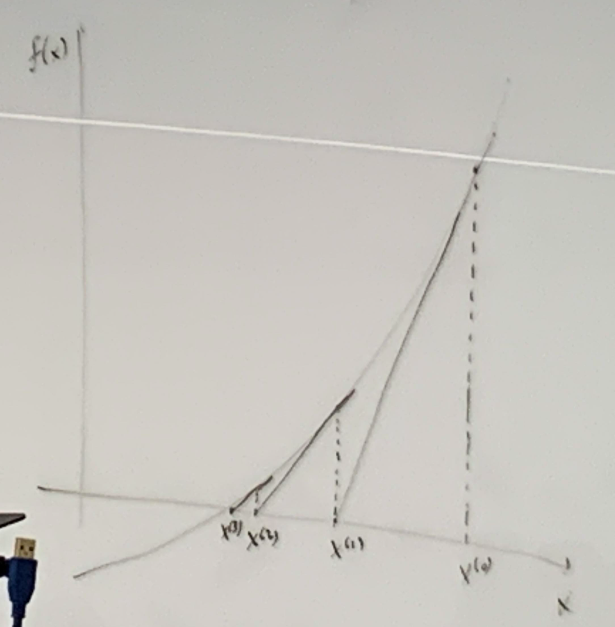
\includegraphics[width = 0.4\linewidth]{Images/410_newtonsmethodinitialguess.png}

    \item Can write iteration as 

    \begin{equation}
        x^{(n+1)} = x^{(n)} - \delta x^{(n)}
    \end{equation}

    \begin{equation}
        f'(x^{(n)}) \delta x^{(n)} = r^{(n)} = f(x^{(n)})
    \end{equation}

    \item Note that we have 

    \[ f'(x^{(n)}) = \frac{f(x^{(n)}}{x^{(n)}-x^{(n+1)}} = \frac{\text{rise}}{\text{run}}\]

\end{itemize}

\textbf{Convergence:} When newton's method converges, does so rapidly, expect number of sig figs to roughly double at each iteration (quadratic convergence).

\vspace{10 px}

\textbf{Example:} "Square Roots"

\begin{equation}
    f(x) = x^2 - a = 0 \qquad \rightarrow \qquad  x^* = \sqrt{a}
\end{equation}

Use other equation

\[ x^{(n+1)} = x^{(n)} - \frac{x^{(n)^2}-a}{2x^{(n)}}\]

\begin{equation}
    \frac{2x^{(n)^2}-(x^{(n)^2}-a)}{2x^{(n)}} = \frac{x^{(n)^2}+a}{2x^{(n)}} = \frac{1}{2} (x^{(n)} + \frac{a}{x^{(n)}}
\end{equation}

\begin{itemize}
    \item Try it with a = 2, 12 digit arithmetic 
    \vspace{10 px}
    Iterate
    \[ x^{(0)} = 1.5\]

    \[ x^{(1)} = \frac{1}{2}(1.5+\frac{2}{1.5}) = 1.416 6666 6667 \qquad \rightarrow \text{3 sig figs}\]

    etc...
\end{itemize}

\subsection{Newton's Method for Systems of equations}

\begin{itemize}
    \item Want to solve
    \[f(x) =0\]

    Where x and f are vectors

    \[x = (x_1 , x_2, ..., x_d)^T\]

    \[ f = (f_1(x), f_2(x),...,f_d(x))^T\]

    Note: Won't always show transpose
    
\end{itemize}

\textbf{Example} (d=2)

\[\sin(xy) = \frac{1}{2}\]

\[ y^2 = 6x+2\]

Ignore fact that we can reduce to d=1 case

Canonical Notation

\[\vec{x}= (x,y)\]

\[ \vec{f} = (f_1(x,y), f_2(x,y))\]

\[ f_1(\vec{x}) = f_1(x,y) = \sin(xy) - \frac{1}{2}\]

\[ f_2(\vec{x}) = f_2(x,y) = y^2 -6x -2 \]

\begin{itemize}
    \item Method again iterate, start from $\vec{x}^{(0)}$

    \item \textbf{Note}: Determining good $x^{(0)}$ more difficult / important than 1-D case;
    Use continuation as necessary
    \item Residual Vector: $\vec{r}^{(n)}$

    \begin{equation}
        \vec{r}^{(n)} = \vec{f}(\vec{x}^{(n)})
    \end{equation}

    \item Analog of f'(x) is Jacobian matric J of first derivatives; elements $J_{ij}$;

    \begin{equation}
        J_{ij} = \frac{\partial f_i}{\partial x_j}
    \end{equation}

    \item Current example

    \[ f_1(x,y) = sin(xy) - \frac{1}{2}\]

    \[ f_2(x,y) = y^2 - 6x -2\]

    \[ \textbf{\underline{\underline{J}}} = \begin{bmatrix}
\frac{\partial f_1}{\partial x} & \frac{\partial f_1}{\partial y} \\

\frac{\partial f_2}{\partial x} & \frac{\partial f_2}{\partial y}
\end{bmatrix} = \begin{bmatrix}
 y \cos{xy} & x\cos{xy} \\
-6 & 2y 
\end{bmatrix}\]
\end{itemize}

\textbf{Newton's Method For Systems of Equations (Continued)}

\begin{itemize}
    \item Derive newton iteration: Multivariate Taylor Series Expansion

    \[ 0 = f(x^*) = f(x^{(n)} + \underline{\underline{J}} [x^{(n)}] \cdot (x^* - x^{(n)} ) + O((x^*-x^{(n)})^2)\]

    Withe Notation: $\underline{\underline{J}} [x^{(n)}] \rightarrow $ Evaluate all Jij's at $x = x^{(n)}$

    \item Drop higher order terms; $x^* \rightarrow x^{(n+1)}$

    \[ 0 = f(x^{(n)} + \underline{\underline{J}} [x^{(n)}] \cdot (x^* - x^{(n)} )\]

    \[ \text{Define } \delta x^{(n)} \equiv - ( x^{(n+1)} - x^{(n)})\]

    \item d-dimensional newton iteration is

    \begin{equation}
        \underline{x}^{(n+1)} = \underline{x}^{(n)} - \underline{\delta x}^{(n)}
    \end{equation}

    Where update vector $\underline{\delta x}^{(n)}$ satisfies dxd linear system

    \begin{equation}
        \underline{\underline{J}}[\underline{x}^{(n)}] \cdot \delta \underline{x}^{(n)} = \underline{f}(\underline{x}^{(n)})
    \end{equation}

    $\rightarrow$ Can be solved in MATLAB using left division operator
    
    \begin{equation}
        J_{ij}[\underline{x}^{(n)}] = \left. \frac{\partial f_i}{\partial x_j} \right|_{\underline{x}=\underline{x}^{(n)}}
    \end{equation}
\end{itemize}

\textbf{General Structure of Newton Solver (PSEUDO CODE HW1!)}

\[x \text{: Solution vector}\]
\[res \text{: Residual vector}\]
\[\underline{\underline{J}} = \text{Jacobian Matrix} \]
\[ dx \text{: Update vector}\]
\[ neq \text{: number of equations}\]

\[ ||v||_2 = rms(v) = \sqrt{\frac{\sum_{i=1}^n v_i^2}{n}} \]


\begin{verbatim}
% x =x^(0)
% while ||dx||_2 > epsilon
%     for i = 1:new
%         res(i) = fi(x)
%         for j = 1:neq
%             J(i,j) = [dfi/dxj](x)
%         end
%     end
%     dx = J \ res % (Linear solve)
%     x = x -dx
% end
\end{verbatim}


\begin{itemize}
    \item Can optimize in MATLAB to not use 2 for loops.

    \item Here and in HW (!!!) should modify above to include code to limit the number of iterations taken (you choose that Number).
    
\end{itemize}

% Missing page